\title{
    \huge{\textcolor{blue!80}{Python与数据结构}} \vspace{0.5cm} \\
    \large{\textcolor{blue!45}{Data Structure}} \vspace{1cm}
    \\ \vspace{2cm}
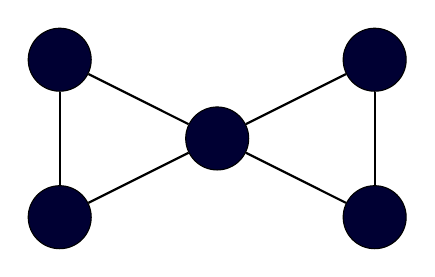
\begin{tikzpicture}[
node/.style = {circle, draw, fill=blue!20!black, inner sep=0pt, minimum size=8mm},
edge/.style = {thick}
]

% 定义节点
\node[node] (A) at (0,0) {};
\node[node] (B) at (2,1) {};
\node[node] (C) at (2,-1) {};
\node[node] (D) at (-2,1) {};
\node[node] (E) at (-2,-1) {};

% 定义边
\draw[edge] (A) -- (B);
\draw[edge] (A) -- (C);
\draw[edge] (A) -- (D);
\draw[edge] (A) -- (E);
\draw[edge] (B) -- (C);
\draw[edge] (D) -- (E);

\end{tikzpicture}
\vspace{4cm}
\\~ \\
}
\author{
	XiaTian \\
	Renmin University of China
}

\pagestyle{empty} % 关闭页码输出
\maketitle
\newpage
~ 
\pagestyle{empty} % 关闭页码输出
